\section{Trim and linearisation}

\subsection{Trimming}
The first step when designing the control system of an aircraft is to study the behavior of the aircraft due to control inputs or external disturbances from an equilibrium condition. If the aircraft we're not to be in equilibrium, deviation from the initial conditions would occur that are unrelated to the control inputs making the analysis more difficult.

In the case of an aircraft this equilibrium condition is known as a trimmed flight condition. In order to determine the trimmed flight condition the states and inputs much be chosen such that the linear- and angular-accelerations are zero. For this assignment this is done by minimizing the following cost function.

\begin{equation}
    \label{eq:trim_cost}
    cost = 5\dot{h}^2 + 
           W_{\phi}\dot{\phi}^2 +
           W_{\theta}\dot{\theta}^2 + 
           W_{\psi}\dot{\psi}^2 +
           2\dot{V_{tot}}^2 + 
           10\dot{\alpha}^2 + 
           10\dot{\beta}^2 + 
           10\dot{P}^2 +
           10\dot{Q}^2 +
           10\dot{R}^2
\end{equation}

All the flight states in the cost function are squared, which is what allows the trim condition to be found by minimizing it. Once the cost function returns zero, the trimmed flight condition states and inputs have been found.

Performing the trimming procedure for 5 iterations in level flight for both flight conditions and both the high and low fidelity models yields the following final values for the cost function.

\begin{center}
    \begin{tabular}{ r | c | c }
                               & high fidelity & low fidelity \\ \hline \hline
     Assigned flight condition & $0.0506$ & $4.2997\cdot10^{-29}$ \\  
     APA flight condition      & $7.1856\cdot10^{-6}$ & $5.1572\cdot10^{-29}$    
    \end{tabular}
\end{center}

The results for the low fidelity models are smaller than the machine epsilon $2.2204\cdot10^{-16}$ of the computer used to calculate these, so it's safe to assume the trimmed flight condition has been successfully found. 

The final cost for the high fidelity model are higher. The results for the APA flight conditions are in the order of $10^{-6}$ and for the assigned flight conditions in the order of $10^{-2}$. This indicates that the resulting state and inputs values are not perfect, but since the cost is close to zero, it may be close enough for further analysis.


\subsection{Accelerometer Position Analysis}
No changes are seen in the $A$ and $B$ matrix after adding the new vertical accelerometer output to the Simulink model. This is expected since the addition of the accelerometer output didn't change the dynamics of the aircraft. However the C and D matrices now have an extra row which corresponds to the new output. Equation~\ref{eq:anss} shows the linearized output equation of the normal acceleration at the center of gravity ($x_a=0$).

\begin{equation}
    \label{eq:anss}
    y = \begin{bmatrix}
        0 \\ 0 \\ -3.24322220018077e-05 \\ 0 \\ -9.67969758700180e-06 \\ 0 \\ 
        0.00398736185031356 \\ 9.92978181907083 \\ 0 \\ 0 \\ 0.966415396225217 \\ 
        0 \\ 0 \\ 0.0208407616972783 \\ 0 \\ 0 \\ 0 \\ 0
        \end{bmatrix}^T x + 
        \begin{bmatrix}
        0 & 0 & 0 & 0
    \end{bmatrix} u
\end{equation}

The accelerometer output primarily depends on the velocity, angle of attack, pitch rate and the normal load factor. The altitude and pitch angle also have a minor contribution, however since it is small these could be caused by errors in the model or linearizion process. Equation~\ref{eq:tf_el_an} shows the transfer function from the elevator to normal acceleration.

\begin{equation}
    \label{eq:tf_el_an}
    \frac{
    \begin{matrix}
        0.421 s^{17} + 22.9 s^{16} + 404.6 s^{15} + 1728 s^{14} - 2.376e04 s^{13} - 3.177e05 s^{12} \\
        - 1.64e06 s^{11} - 5.127e06 s^{10} - 1.168e07 s^{9} - 1.574e07 s^{8} - 7.901e06 s^{7} \\
        - 5.914e04 s^{6} +  746.3 s^{5} + 4.87 s^{4} - 1.464e-11 s^{3}
    \end{matrix}
    }{
    \begin{matrix}
        s^{18} + 80.51 s^{17} + 2581 s^{16} + 4.234e04 s^{15} + 3.876e05 s^{14} + 2.115e06 s^{13} \\
        + 7.644e06 s^{12} + 2.059e07 s^{11} + 3.952e07 s^{10} + 5.029e07 s^{9} + 4.057e07 s^{8} \\
        + 1.553e07 s^{7} + 5.631e05 s^{6} + 1.073e05 s^{5} + 1159 s^{4} - 8.86e-11 s^{3}
    \end{matrix}
    }
\end{equation}

The transfer function has a zero on the right hand side of the imaginary axis at $9.76+0j$. This zero is the one responsible for the non-minimum-phase behavior. The physical explanation of this is that a pitch up maneuverer with the elevator produces a downwards force which causes the aircraft to accelerate downwards. Eventually the angle of attack will increase as the nose pitches up and the extra lift will accelerate the aircraft upwards.

\begin{figure}[ht]
    \centering
    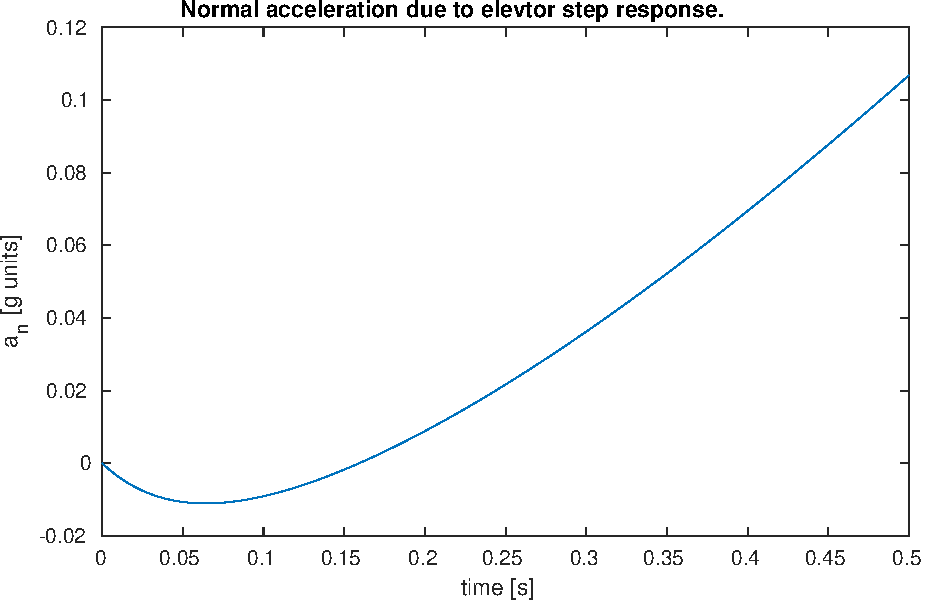
\includegraphics[width=0.6\textwidth]{figures/an_elev_step}
    \label{fig:an_elev_step}
    \caption{Normal acceleration after a negative step input on the elevator.}
\end{figure}

Repeating the simulation for increasing values of $x_a$ shows that the zero moves away from the origin indicating that its influence becomes less dominant. When $x_a=5.9$ the zero has moved to the left side of the imaginary axis and the non-minimum-phase behavior disappears. Since the value of the zero is significantly larger than that the other zeros and poles, its motion is negligible. Increasing $x_a$ further moves the zero closer to origin and its motion reappears, this time in the direction of the reference signal.

\begin{figure}[ht]
    \centering
    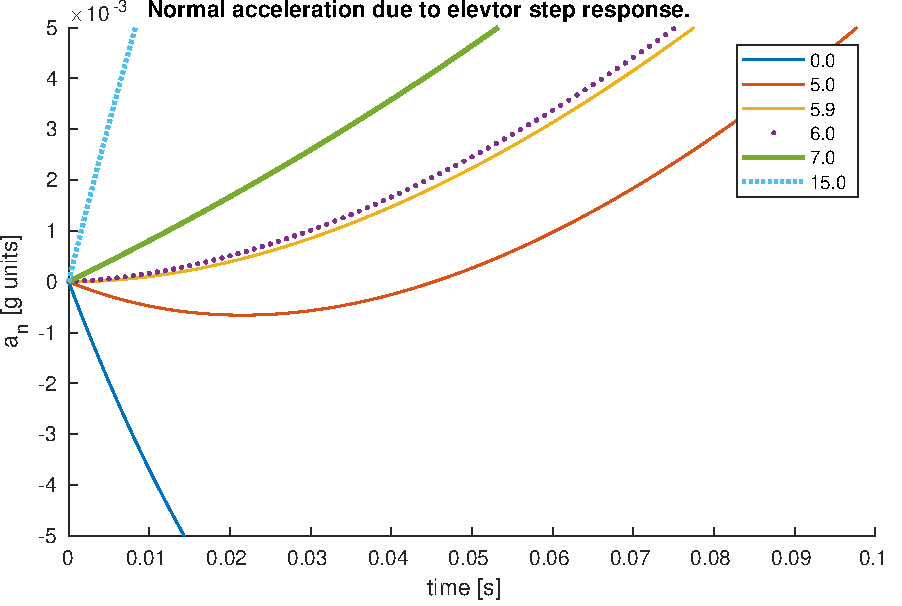
\includegraphics[width=0.6\textwidth]{figures/an_elev_step_mult}
    \caption{Normal acceleration after a negative step input on the elevator for different values of $x_a=5.9$.}
    \label{fig:an_elev_step_mult}
\end{figure}

One property of the \emph{instantaneous center of rotation} is that the linear accelerations at that point are the same as that of the overall aircraft. A point in front of it will accelerate upwards with a pitch up manoeuvre and a point behind it will accelerate downwards during the same manoeuvre. Thus based on the effects of moving $x_a$, it fair to conclude that the instantaneous center of rotation must be near $x=5.9$. Another way to arrive at the same conclusion is that the acceleration due to rotation is caused by the zero mentioned in the previous section since this is the only zero that changes significantly with $x_a$. Thus the instantaneous center of rotation will be at the location where this zero is infinitely far away from the origin.

The pilot should be placed at or after the instantaneous center of rotation ($x_a\geq5.9\ ft$), this is because if he is placed before, he will initially feel the aircraft moving into the opposite direction he is commanding it to and this might confuse the pilot resulting in him compensating for an error that is not there. This could make the combined human-aircraft system unstable or at least difficult to control.

It is important to place the accelerometer close a node of the most important fuselage bending moment. The reason is because, as the aircraft flies, loads and vibrations acting on the aircraft will make the fuselage bend. The nodes are locations where the displacements due to vibrations or bending are zero. Thus placing the accelerometer far away from a node, will result in the accelerometer measuring extra accelerations due to vibrations or bending. 


\clearpage
